\documentclass[a4paper,11pt]{extarticle} % тип документа
\usepackage[left=1.6cm,right=1.6cm]{geometry}
%%%Библиотеки
    %\usepackage[warn]{mathtext}	
    \usepackage[T2A]{fontenc}   %Кодировка
\usepackage[utf8]{inputenc} %Кодировка исходного текста
    \usepackage[english, russian]{babel} %Локализация и переносы
    \usepackage{caption}
    \usepackage{listings}
    \usepackage{amsmath, amsfonts, amssymb, amsthm, mathtools}
    \usepackage[warn]{mathtext}
    \usepackage[mathscr]{eucal}
    \usepackage{wasysym}
    \usepackage{graphicx} %Вставка картинок правильная
    \usepackage{indentfirst}
    \usepackage{float}    %Плавающие картинки
    \usepackage{wrapfig}  %Обтекание фигур (таблиц, картинок и прочего)
    \usepackage{fancyhdr} %Загрузим пакет
    \usepackage{lscape}
    \usepackage{xcolor}
    \usepackage[normalem]{ulem}
        \usepackage{multirow}

    \usepackage{titlesec}
    \titlelabel{\thetitle.\quad}


%%%Конец библиотек


%Заголовок
\title{Отчет о выполнении лабораторной работы 3.4.5 \\ 
\textbf{Петля гистерезиса (динамический метод)}}
\author{Севастьян Черняков}
\date{ ФУПМ МФТИ, 2023 \\}
\begin{document}
\maketitle 





\section{Введение}

\textbf{Цель работы:} 

	Изучение петель гистерезиса различных ферромагнитных
материалов в переменных полях.


\textbf{В работе используются:} 

Автотрансформатор, понижающий трансформатор, интегрирующая цепочка, амперметр, вольтметр, электронный
осциллограф, делитель напряжения, тороидальные образцы с двумя обмотками.





	
\section{Результаты измерений и обработка данных}


\subsection{Исследование петли гистерезиса}
Параметры установки следующие: $R_0 = 0.3 \; \text{Ом}$, $R_{\text{и}} = 20 \; \text{кОм}$, $C_{\text{и}} = 20 \; \text{мкФ}$, $\omega = 50\text{Гц}$. Подберем ток питания в намагничивающей обмотке с помощью автотрансформатора и коэффициенты усиления ЭО таким образом, чтобы предельная петля гистерезиса занимала большую часть экрана. Приведем характерные значения катушек разных материалов в таблице .


\begin{table}[h]
	\centering
	\begin{tabular}{|l|l|l|l|}
		\hline
		& Феррит & Пермаллой & Крем. железо \\ \hline
		$N_0$          & 35     & 35        & 35                \\ \hline
		$N_U$          & 400    & 220       & 350               \\ \hline
		$S$, $\text{см}^2$    & 3      & 3.8       & 1.2               \\ \hline
		$2\pi R$, $\text{см}$ & 25     & 24        & 10                \\ \hline
	\end{tabular}
	\caption{Параметры образцов}
	\label{new}
\end{table}

Для каждого образца получим передельные петли гистерезиса, по коэффициентам усиления ЭО $K_x$ и $K_y$ рассчитаем масштабы, определим двойные амплитуды коэрцетивной силы $ [2x(c)] $ и индукции насыщения $ [2y(s)] $. Здесь $K_x = 2R_0\sqrt2I_{\text{эф}}/2x$, $K_y = 2\sqrt 2 U_{\text{эф}}/2y$. Масштабы по осям $ X $ и $ Y $ рассчитаем по формулам 
$H=IN_0/(2\pi R)$, где $I=K_x/R_0;\ B=R_\text{и}C_\text{и}U_{\text{вых}}/(SN_\text{и}),$ $U_{\text{вых}}=K_y$. 


Для феррита:
\begin{equation*}
	H = \frac{K_x N_0}{2 \pi R R_0} = \frac{0.02 * 35}{0.25*0.3} = 9.3 \pm 0.9 \; \text{\text{(А / м) / дел}},
\end{equation*}
\begin{equation*}
	B = \frac{R_\text{И} C_\text{И} K_y}{S N_\text{И}} = \frac{20000 * 20*10^{-6} * 0.02}{3*10^{-4}*400} = 0.067\pm 0.007 \; \text{\text{Тл / дел}}.
\end{equation*}

Для пермаллоя:
\begin{equation*}
	H = \frac{0.02 * 35}{0.24 * 0.3} = 10\pm 1\; \text{(А / м) / дел},
\end{equation*}
\begin{equation}
	B = \frac{20000 * 20*10^{-6} * 0.02}{3.8 * 10^{-4} * 220} = 0.1\pm 0.01\; \text{Тл / дел}.
\end{equation}

Для кремнистого железа:
\begin{equation*}
	H = \frac{0.1 * 35}{0.1 * 0.3} = 120 \pm 10 \; \text{(А / м) / дел},
\end{equation*}
\begin{equation*}
	B = \frac{20000 * 20*10^{-6} * 0.1}{1.2 * 10^{-4} * 350} = 1.0\pm 0.1 \; \text{Тл / дел}.
\end{equation*} 


Далее, найдём индукцию насыщения - максимальную индукцию, которую можно получить в данном магнитном материале, и коэрцитивную силу - значение напряжённости внешнего магнитного поля, необходимое для полного размагничивания ферромагнитного вещества..

Для феррита:
\begin{equation*}
	H_c = \frac{(2x_c) * H}{2} = 3.1 * 9.3 / 4 = 15.0 \pm 0.1 \; \text{А/м},
\end{equation*}
где $ H $ -- цена деления для $ K_x = 5 \; mV $.
\begin{equation*}
	B_s = \frac{(2 y_s) * B}{2} = 2.1 * 0.067 = 0.143 \pm 0.005 \; \text{Тл}.
\end{equation*}
Тогда амплитуда, соответствующая состоянию насыщения $H_s = 30.3 \pm 0.9$ \text{А/м}, индукция насыщения в этом случае $B_r = 0.069\pm 0.007$ Тл 

Для пермаллоя:
\begin{equation*}
	H_c = 3.1 * 9.7 = 30.1 \pm 0.1 \; \text{А / м}
\end{equation*}
\begin{equation*}
	B_s = 2.9 * 5 * 0.095 = 1.45 \pm 0.03 \; \text{Тл}
\end{equation*}
Также для пермаллоя $H_s = 64 \pm 2$ \text{А/м}; $B_r = 1.02\pm 0.06$ Тл

Для кремнистого железа:
\begin{equation*}
	H_c = 3 * 116 / 5 = 69.5 \pm 0.2 \; \text{А / м}
\end{equation*}
\begin{equation*}
	B_s = 3 * 0.95 / 2 = 1.43 \pm 0.03 \; \text{Тл}.
\end{equation*}

Также для кремнистого железа $H_s = 430 \pm 10$ \text{А/м}; $B_r = 0.62\pm 0.08$ Тл


Табличные данные для исследуемых материаов приведены ниже.



Сравнивая полученные данные с табличными, можно утверждать, что они совпадают лишь по порядку величины.

Также приведём фотографии предельных петель гистерезиса.


По начальным кривым намагничивания и найдем, чему равны начальное и максимальное значения дифференциальной магнитной проницаемости 
$\mu_{\text{диф}} = dB/dH$. Получим следующие значения: $\mu_{\text{нач}} \approx 750, \; \mu_{max} \approx 290$ для феррита, 
$\mu_{\text{\text{нач}}} \approx 1300,\; \mu_{max} \approx 3700$ для пермаллоя и  $\mu_{\text{нач}} \approx 430, \; \mu_{max} \approx 6800$ для кремнистого железа.


\begin{figure}[H]
    \centering
    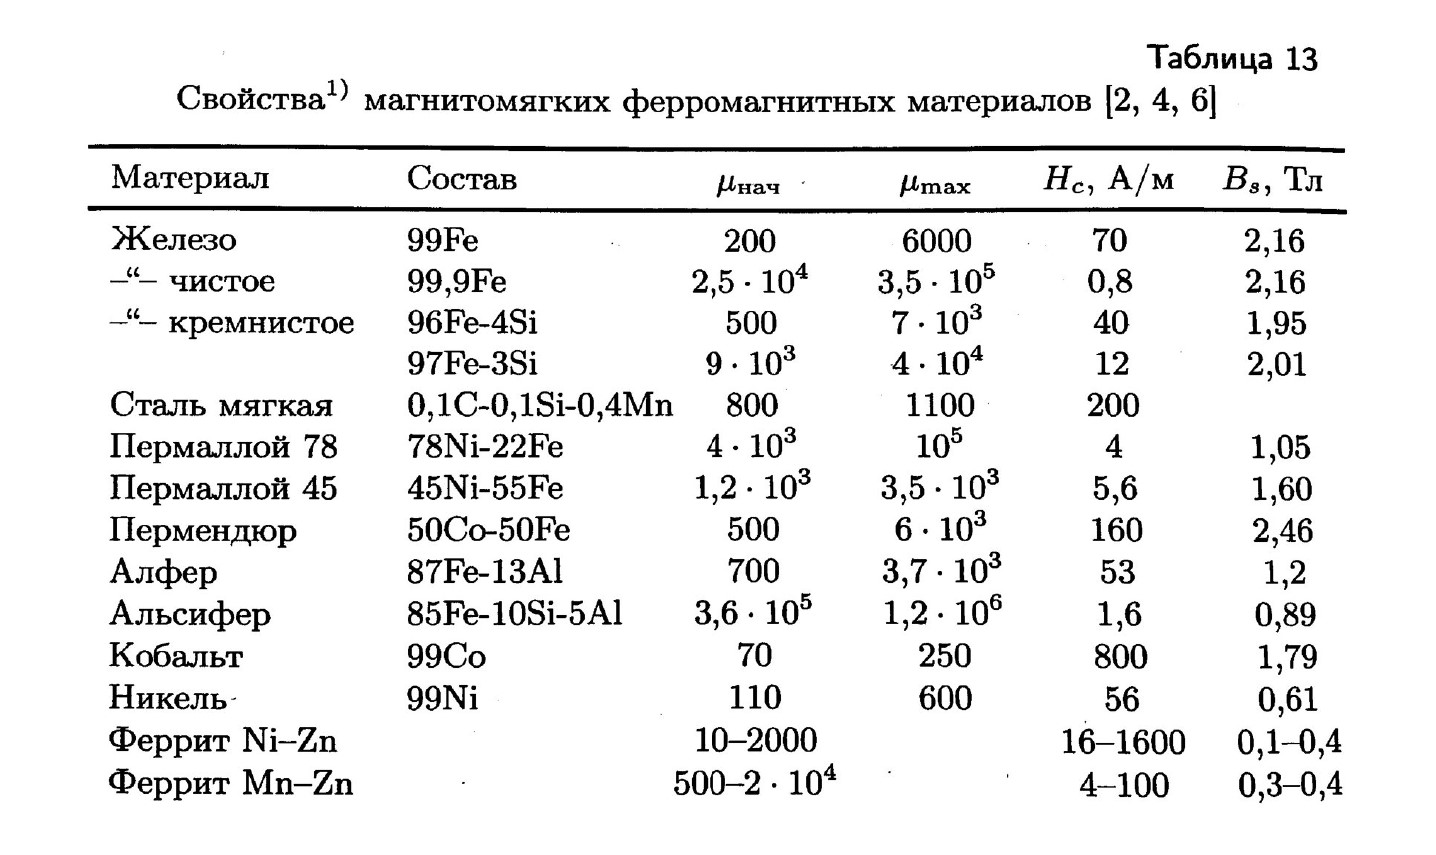
\includegraphics[width = 15 cm]{Таблица 13_page-0001.jpg}
    \caption{Свойства магнитомягких ферромагнитных материалов}
\end{figure}

\begin{figure}[H]
    \centering
    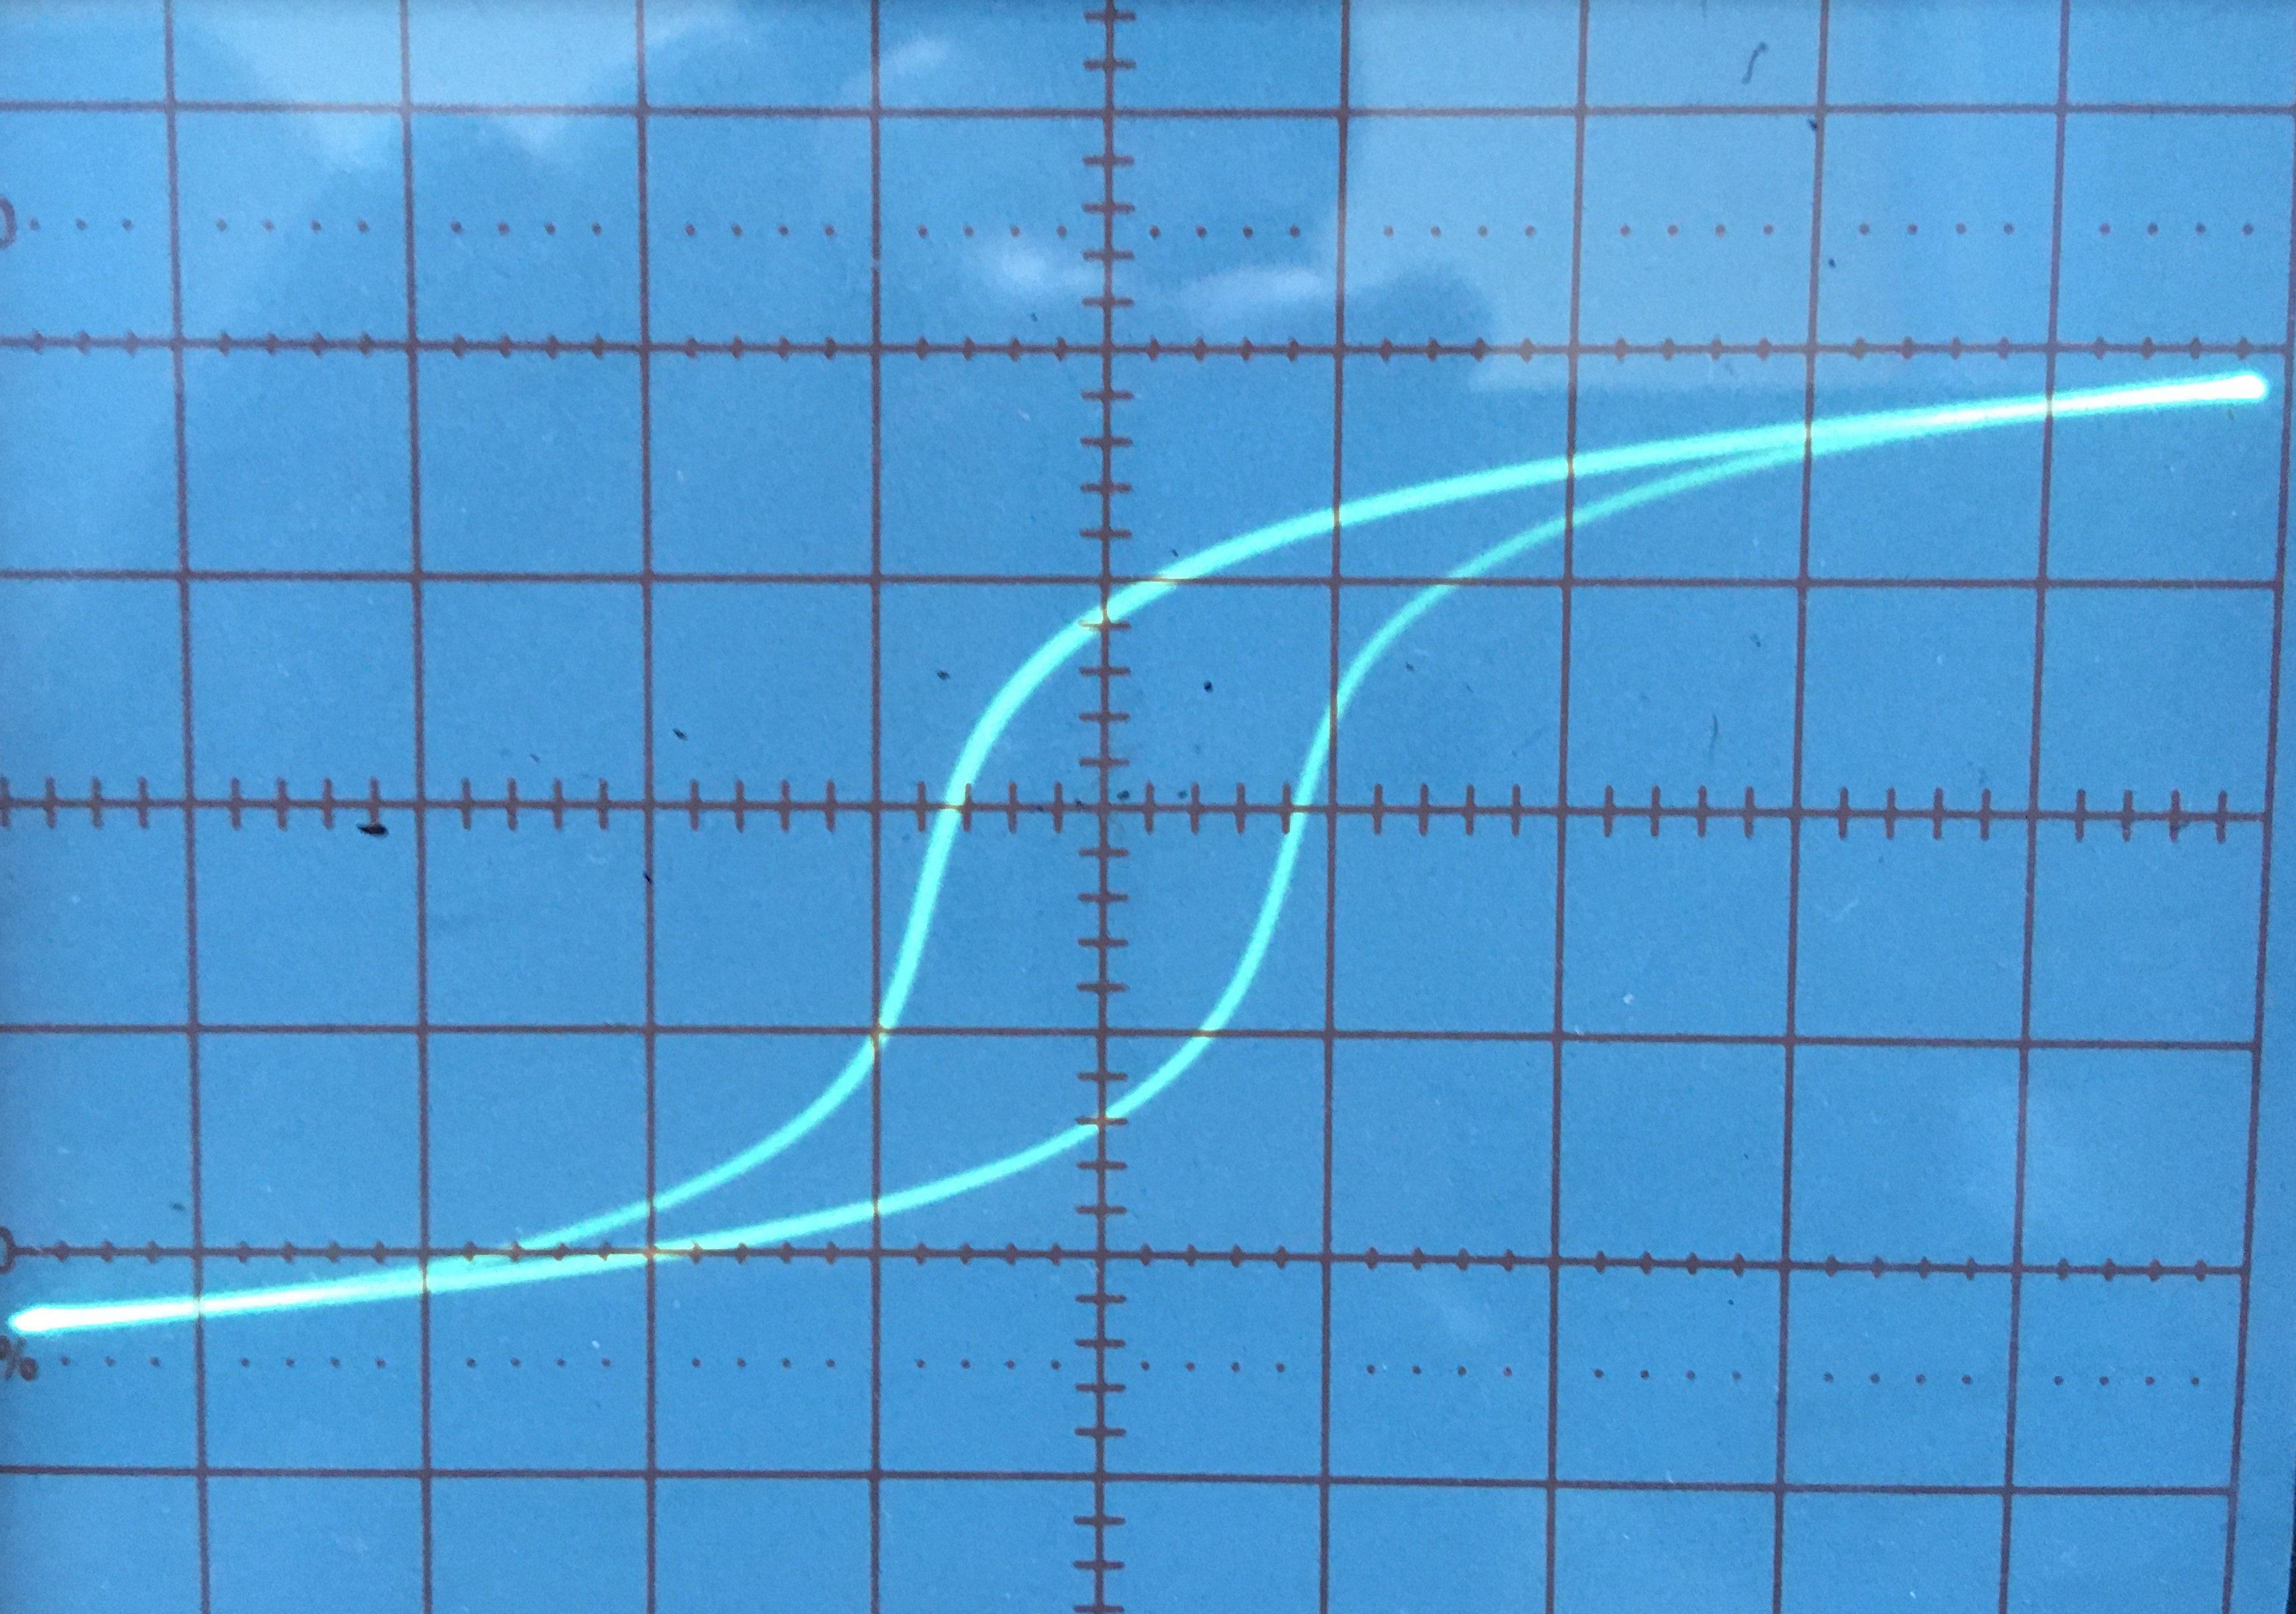
\includegraphics[width = 15 cm]{Феррит.JPG}
    \caption{Предельная петля гистерезиса феррита}
\end{figure}


\begin{figure}[H]
    \centering
    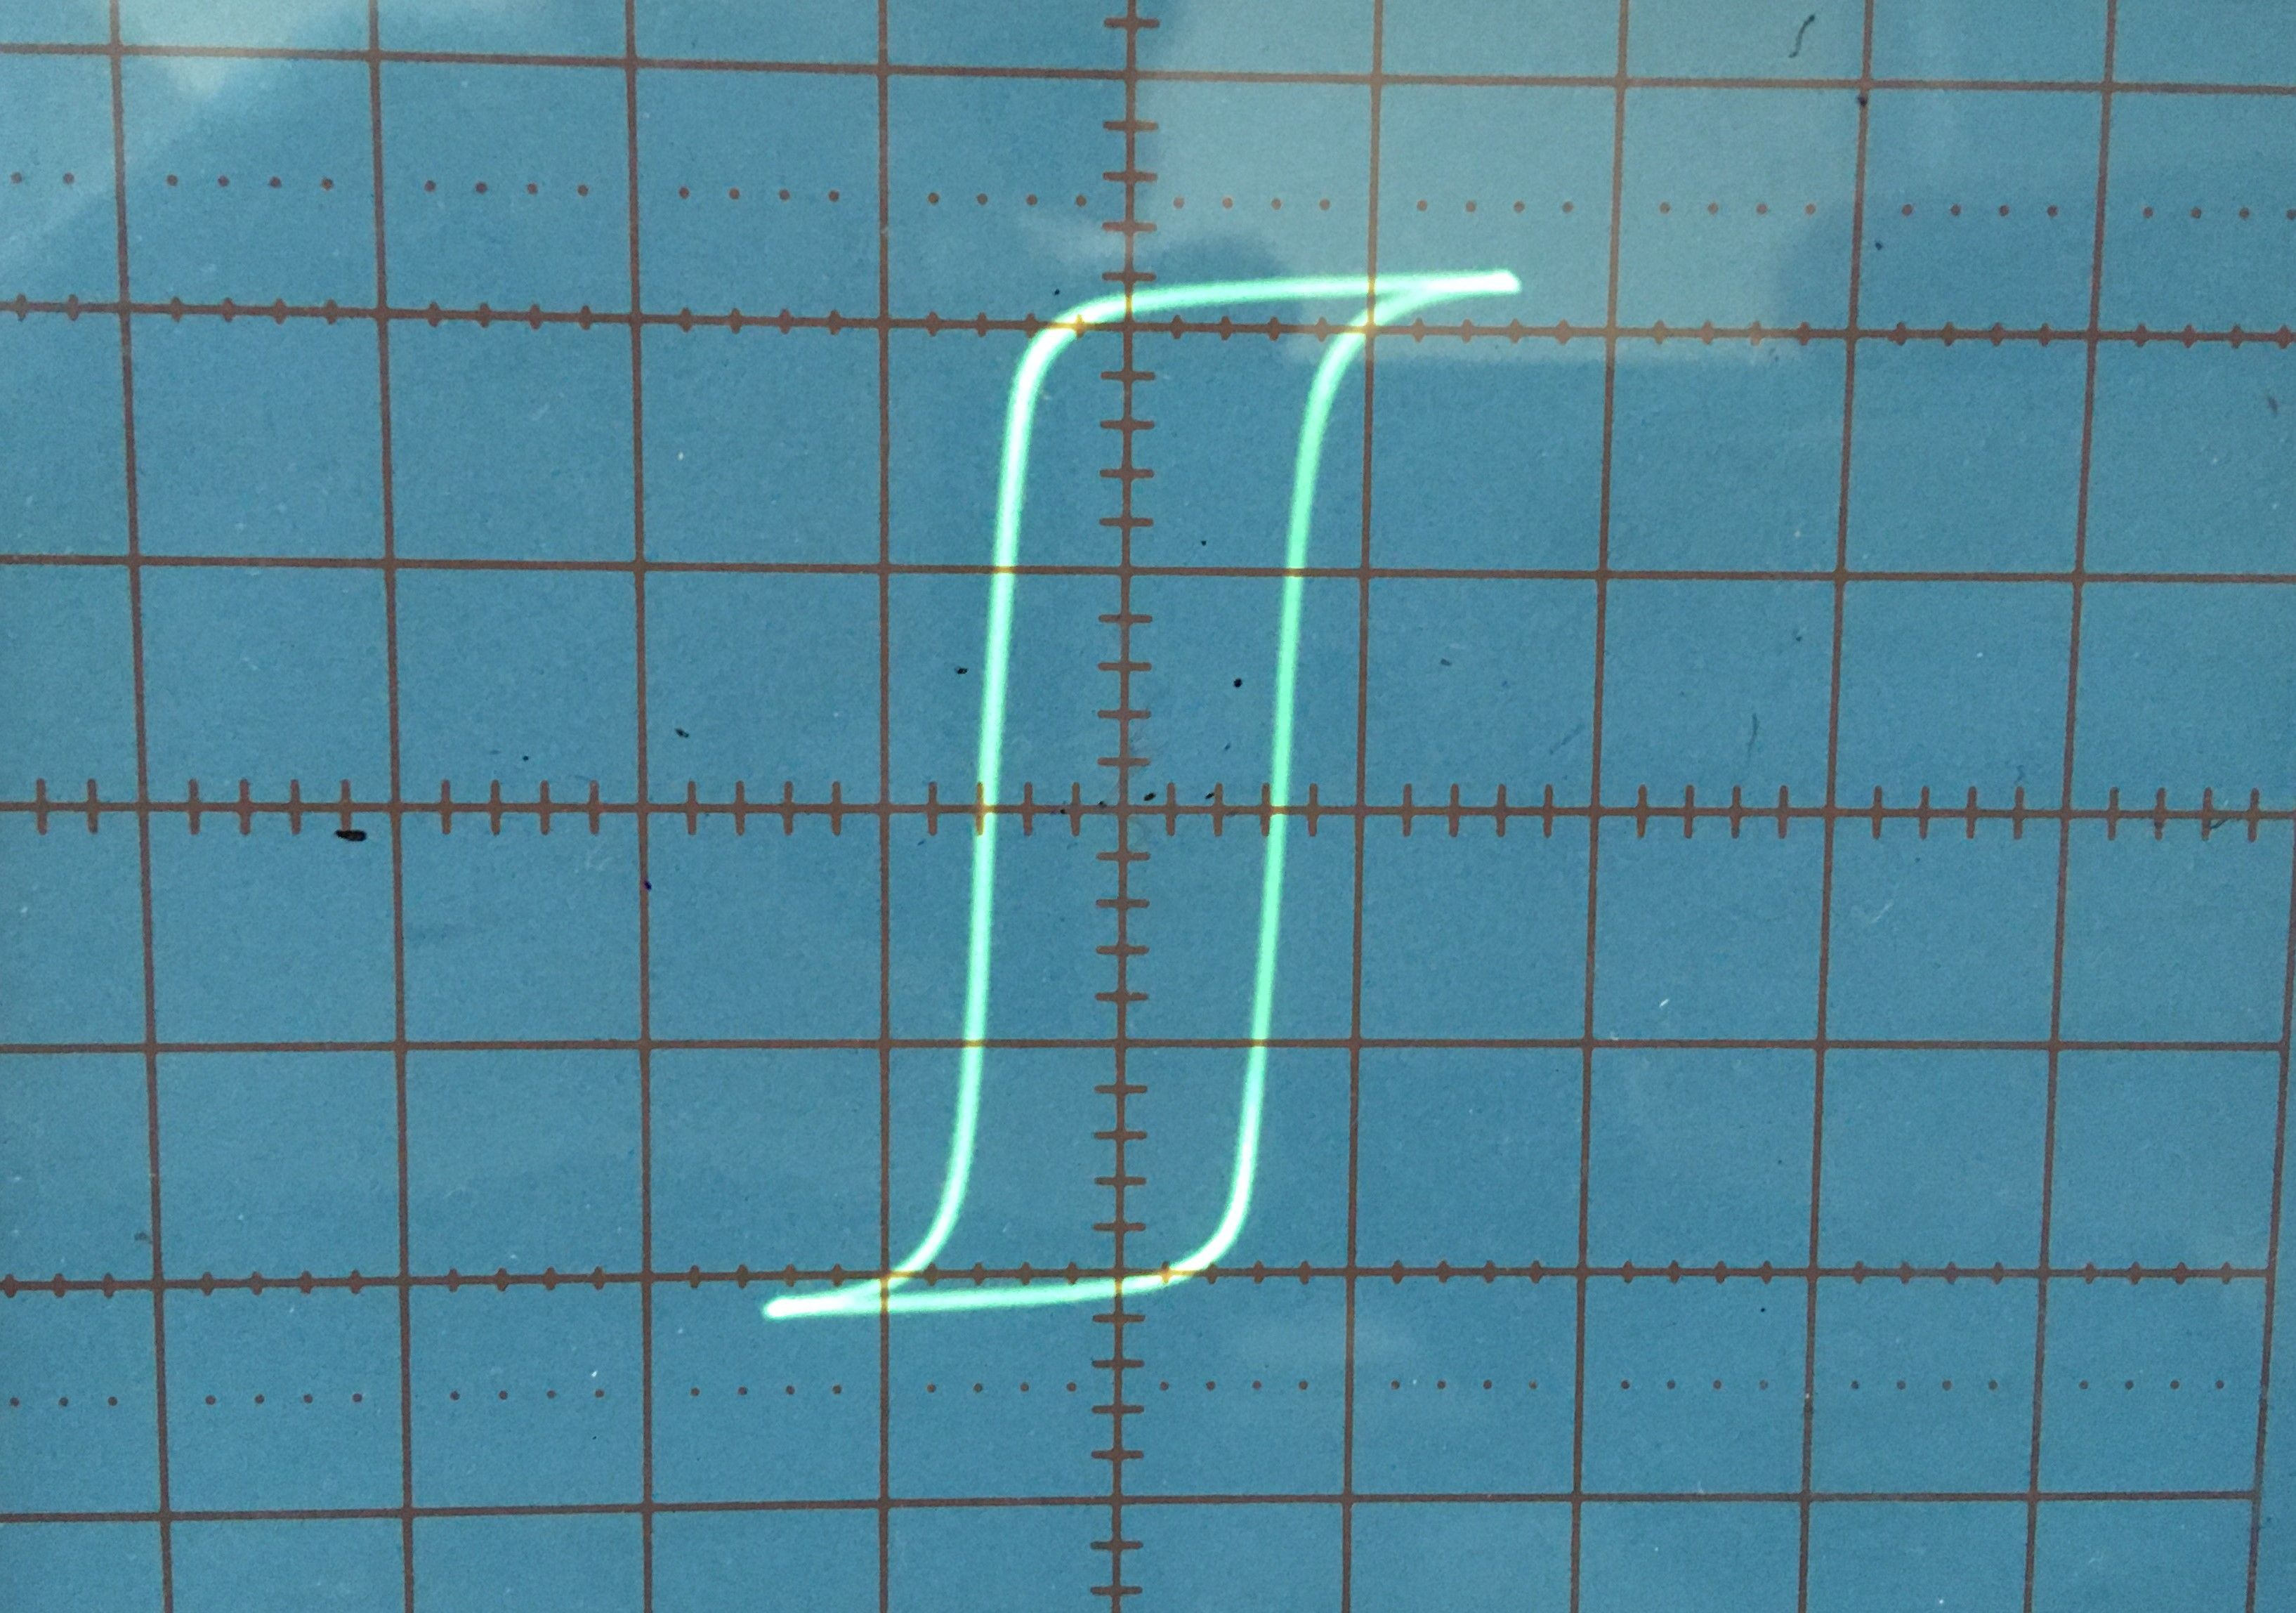
\includegraphics[width = 15 cm]{Пермаллой.JPG}
    \caption{Предельная петля гистерезиса пермаллоя}
\end{figure}


\begin{figure}[H]
    \centering
    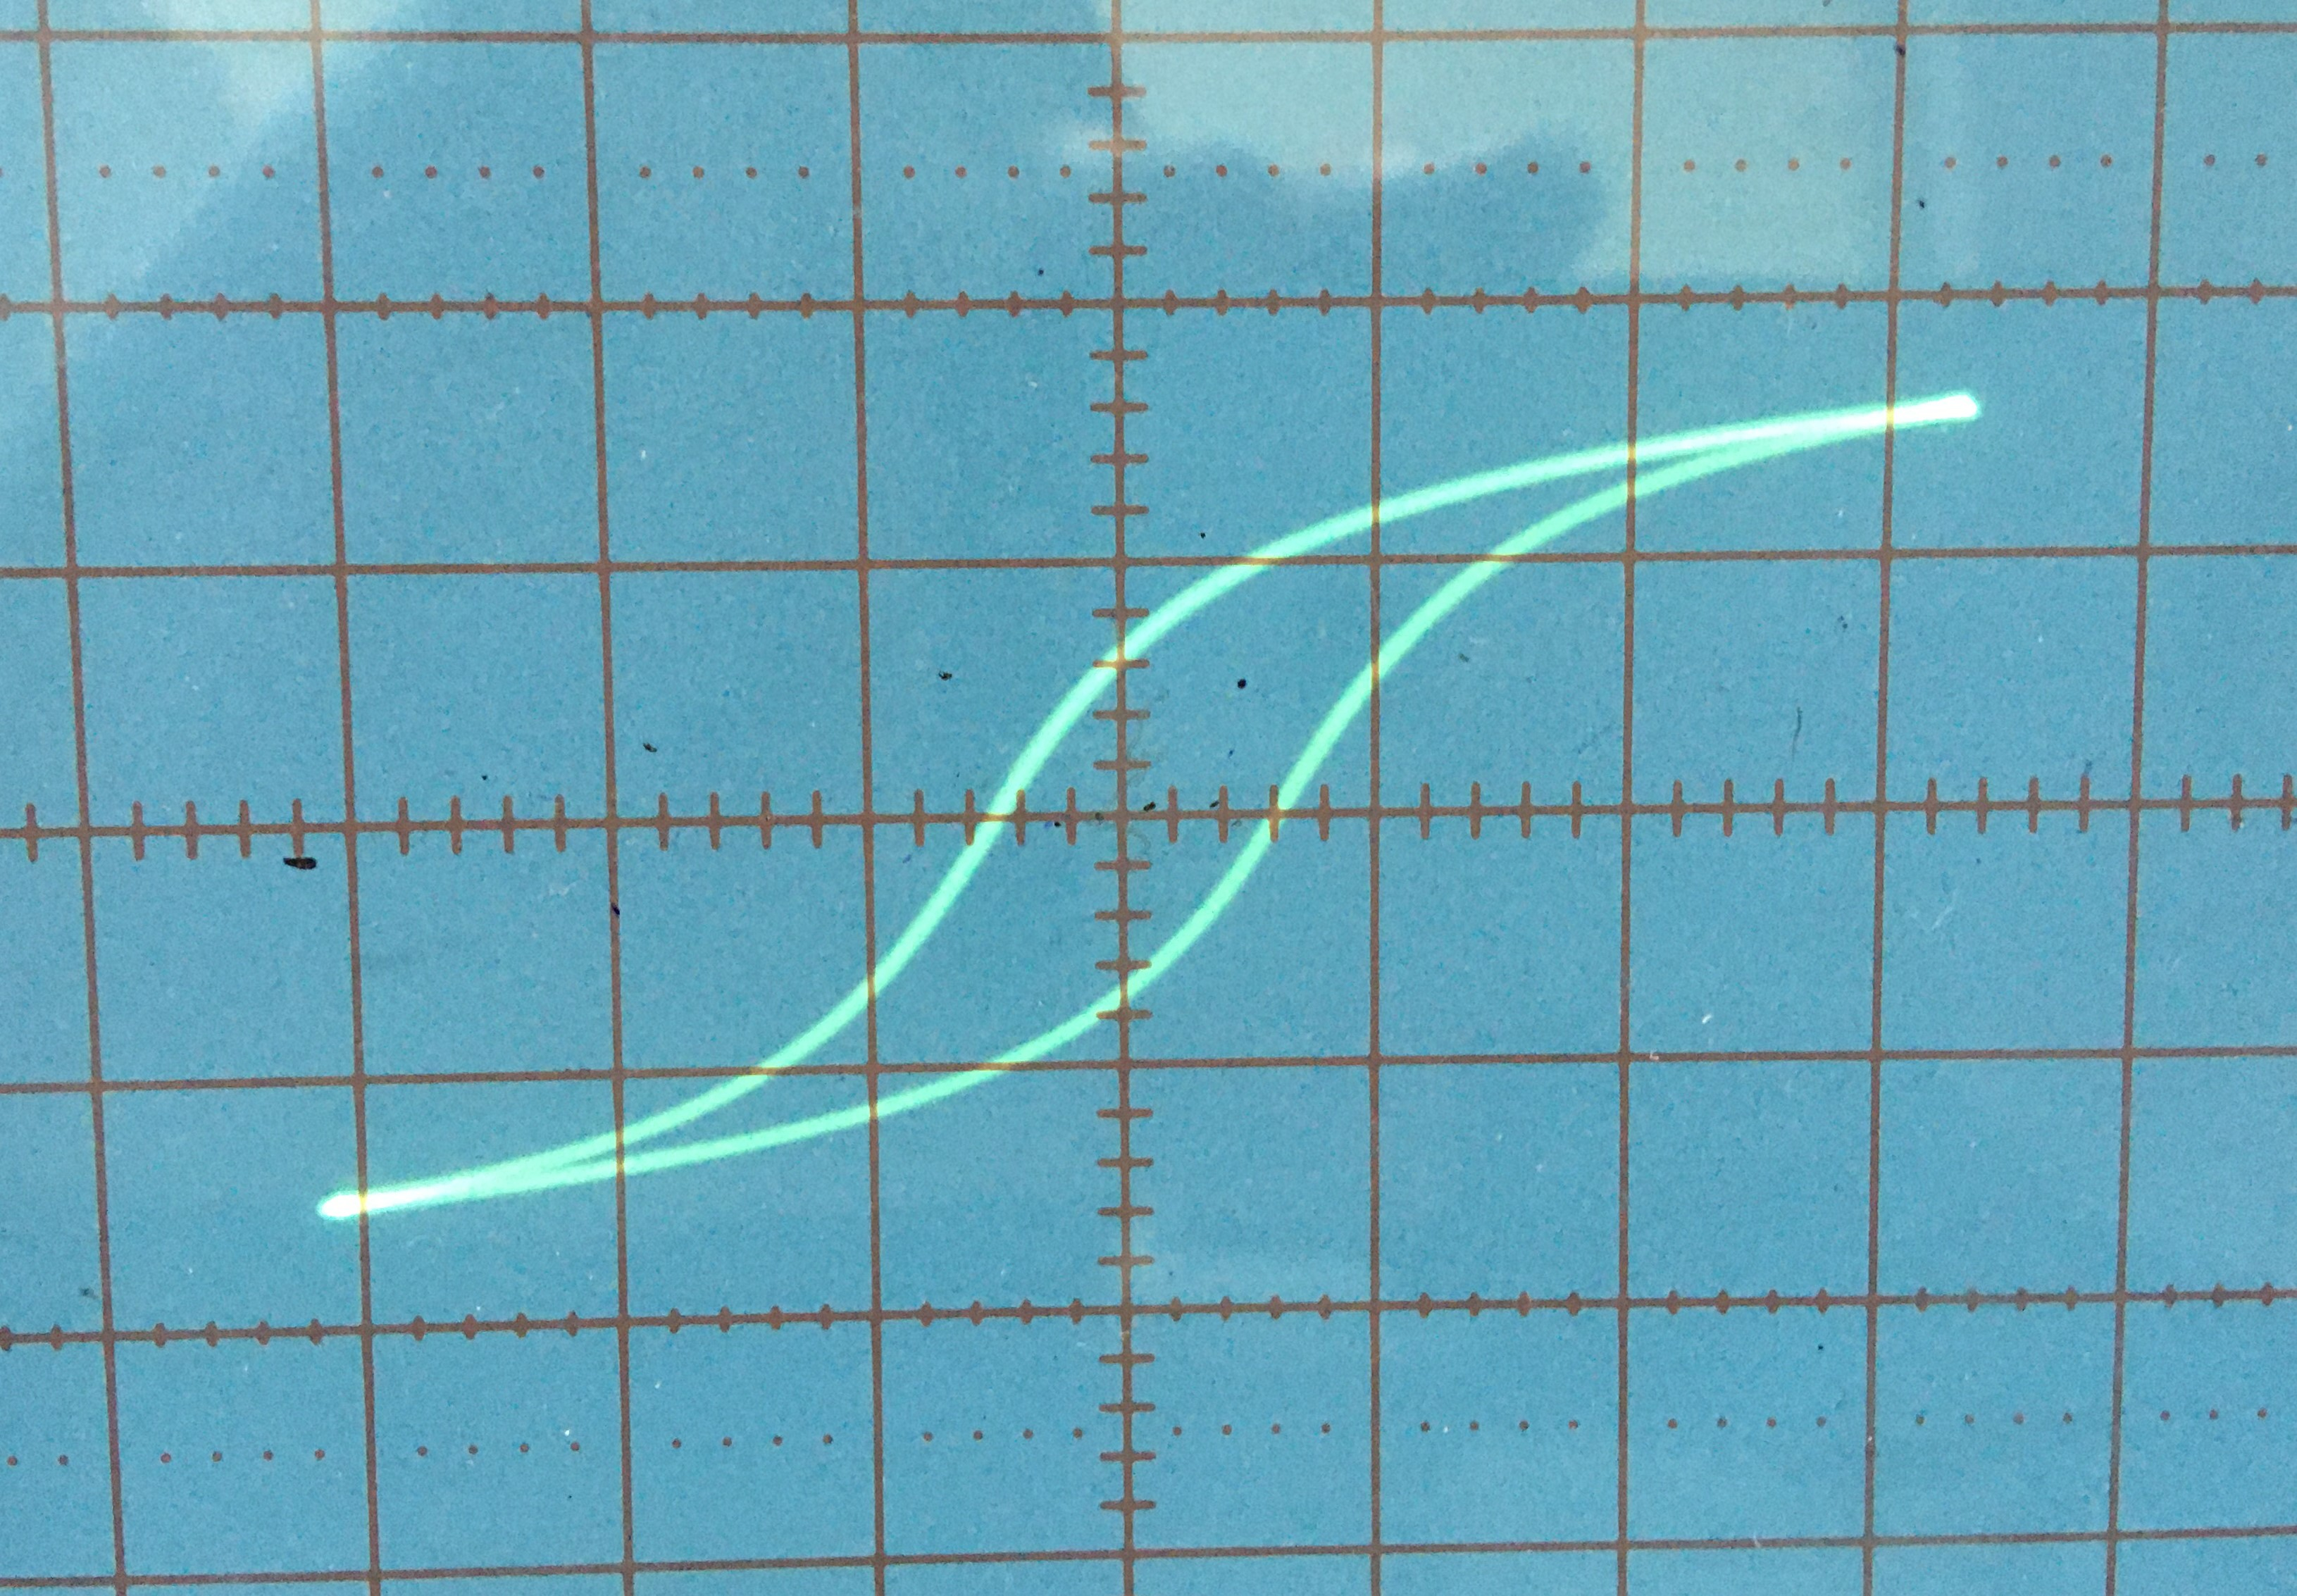
\includegraphics[width = 15 cm]{Кремнистое.JPG}
    \caption{Предельная петля гистерезиса крменистого железа}
\end{figure}



\subsection{Проверка калибровки осциллографа}

Проверим калибровку ЭО по оси X. Отключим намагничивающую обмотку $N_0$ от цепи, соединив оба провода, идущих к обмотке, на одной ее клемме. С помощью автотрансформатора подберем такой ток через $R_0$, при котором горизонтальная прямая занимает большую часть экрана. При $ K_x=0,1 \text{ В/дел} $ рассчитаем чувствительность $m_x=0,098 \text{ В/дел}$.

Аналогичные действия проводим при $ K_x =0,05 \text{ В/дел} $. Получаем $ m_x=0,049 \text{ В/дел} $  .

Так как $m_x \approx K_x$, ЭО откалиброван по оси X корректно.

Также необходимо проверить калибровку по оси $ Y $. Для этого соединим вход Y ЭО с клеммам делителя "1:100 - земля". Не меняя рабочего коэффициента $K_y = 0,05\text{ В/дел}$, подберем с помощью трансформатора напряжение, при котором вертикальная прямая занимает большую часть экрана. Подключим вольтметр V к тем же клеммам делителя и, используя измеренное $U_{\text{эф}}$, рассчитаем чувствительность $m_y=0,048\text{ В/дел}$.

Те же действия повторяем при $K_y = 0,02\text{ В/дел}$. Получаем $m_y=0,019\text{ В/дел}$.

Так как $m_y \approx K_y$, ЭО откалиброван по оси Y корректно.


\subsection{Определение 4$\tau$ - постоянной времени интегрирующей ячейки}
Проверим применимость формулы (2). Для этого рассчитаем $\tau$ -- постоянную времени $ RC $-цепочки. 
Для определения напряжений на входе и выходе интегрирующей ячейки соединим вход ячейки с обмоткой <<6,3 В>> трансформатора.
Подключим Y-вход ЭО ко входу интегрирующей ячейки и отключим X-вход ЭО. Подберем такой ток, чтобы вертикальная прямая занимала большую часть экрана,
и определим входное напряжение $U_{\text{вх}}=2y\cdot K_y=5,6\ \text{дел} \cdot 1\ \text{В/дел}=5,6\ \text{В}$. 
Не меняя тока, подключим Y-вход ЭО к выходу ячейки и аналогичным образом определим $U_{\text{вых}}=2y\cdot K_y=0,004\ \text{В}$. Рассчитаем $\tau_{\text{эксп}}:$


\begin{equation*}
	\tau_{\text{эксп}} = \frac{U_{\text{вх}}}{\omega U_{\text{вых}}} = \frac{5.6}{2 \pi * 50 * 0.04} = 0.44\pm 0.01 \; c
\end{equation*}


По определению $\tau_{RC}=R_\text{и}C_\text{и}=0,4\ \text{с}$.

$\tau_{\text{теор}} = R C = (20*10^3)*(20*10^{-6}) = 0.4\; \text{c}$




\section{Вывод}

% Please add the following required packages to your document preamble:
% \usepackage{multirow}
% Please add the following required packages to your document preamble:
% \usepackage{multirow}
Многие характеристики отличаются от справочных. Связано это, во-первых, с несовершенством исследуемого метода (например, снятия показаний с осциллографа), во-вторых, 
с разной концентрацией металлов в разных сплавах. Тем не менее, оценочно удалось определить некоторые магнитные параметры данного ряда веществ.

\begin{table}[h]
	\centering
	\begin{tabular}{|l|l|l|l|}
		\hline
		Ампл.                          & Феррит           & Fe-Ni           & Fe-Si          \\ \hline
		\multirow{2}{*}{$H_\text{c}, \; \text{А/м}$} & $15\pm 0.1$      & $30.1\pm 0.1$   & $69.5\pm 0.2$  \\ \cline{2-4} 
		& $4-100$             & $5.6$       & $40$          \\ \hline
		\multirow{2}{*}{$B_s, \text{Тл}$}     & $0.143\pm 0.005$ & $1.45\pm 0.03$  & $1.43\pm 0.03$ \\ \cline{2-4} 
		& $0.3 - 0.4$           & $1.6$   & 2.01              \\ \hline
		\multirow{2}{*}{$\mu_{max}$}     & $290$ & $3700$  & $6800$ \\ \cline{2-4} 
		& $-$           & $(3.5) \cdot 10^3$   & $7\cdot 10^3$             \\ \hline
		
		\multirow{2}{*}{$\mu_{\text{нач}}$}     & $750$ & $1300$  & $430$ \\ \cline{2-4} 
		& $10 - 2000 / 500 - 2\cdot 10^4$           & $(1.2 - 4)\cdot 10^3$   & 500 - 9000              \\ \hline
		
		
	\end{tabular}
	\caption{Сводная таблица магнитных характеристик (табичные внизу)}
	\label{tab:my-table}
\end{table}

\end{document}\end{document}